\documentclass[preprint, hmargin=1in, vmargin=1in]{aastex62}
%%%%%%begin preamble
%\usepackage[hmargin=1in, vmargin=1in]{geometry} % Margins
\usepackage{hyperref}
\usepackage{url}
\usepackage{natbib}
\setlength{\bibsep}{0pt plus 0.3ex}
\usepackage{graphicx}
\usepackage{amsmath}
\usepackage{amsfonts}
\usepackage{amssymb}
%\usepackage{import}
\usepackage{wrapfig}
\usepackage{changepage}
\usepackage{lipsum}

\usepackage{color}
\hypersetup{
  colorlinks   = true,
  %citecolor    = blue
  citecolor    = gray
  % gray is not being found!?!
  % gray is found if pdfpages is used... crap.
  %citecolor    = grey
  %citecolor    = Gray
}

%% headers
\usepackage{fancyhdr}
\pagestyle{fancy}
\fancyhf{} % sets both header and footer to nothing
\lhead{Evan Anders -- Research Statement}
\rhead{KITP Postdoctoral Scholar Position with Prof.~Bildsten}
\cfoot{\footnotesize{\thepage}}
%\pagestyle{empty}
%\pagenumbering{gobble}
%\renewcommand*{\thefootnote}{\fnsymbol{footnote}}

\renewcommand{\vec}{\ensuremath{\boldsymbol}}
\newcommand{\dedalus}{\href{http://dedalus-project.org}{Dedalus}}
\newcommand{\del}{\ensuremath{\vec{\nabla}}}
\newcommand{\scrS}{\ensuremath{\mathcal{S}}}

\newcommand{\prf}{Physical Review Fluids}

\begin{document}
\maketitle
\vspace{-88pt}
\section*{\textbf{Research Interests and Plans}}
\thispagestyle{fancy}
Asteroseismology has undergone a revolution in the past decade thanks to the wealth of space-based photometric data now available from missions like CoRoT and \emph{Kepler} \citep{huber&all2019}.
Asteroseismic interpretation of data often relies on stellar structure models, such as those produced by state-of-the-art codes like MESA \citep[e.g.,][]{paxton&all2011, paxton&all2019}.
One limitation of these 1D structure models is that they depend on 1D parameterizations like mixing length theory \citep[MLT,][]{bohm-vitense1958} to describe convection.
MLT does an adequate job of describing heat transport by stellar convection, but also assumes that convection zones generate flows at all radial locations with length scales proportional to the atmospheric scale height.
MLT thus predicts that stars with convective envelopes should drive large-scale ``giant cells'' beneath smaller-scale, near-surface convective cells. 
Giant cells have not been detected in direct measurements of flows at the Sun's photosphere \citep{hathaway&all2015} or in helioseismic observations \citep{hanasoge&all2015}; this disagreement between theory and observations is referred to as the ``Solar Convective Conundrum.''
%We must solve this Convective Conundrum in order to improve stellar structure models and asteroseismic measurements of stars with convective envelopes.
In my research, I use the Dedalus code \citep{burns&all2019} to create simulations of stellar convection to help solve the Convective Conundrum.
As a postdoctoral researcher at KITP, I will utilize MESA and Dedalus to explore how the Convective Conundrum affects stellar structure.
These explorations will specifically examine how stellar structure is affected by \emph{nonlocal heat transport processes in convection} and by \emph{replacing MLT-like parameterizations with statistics from 3D simulations}.

\section*{\textbf{Entropy Rain: Nonlocal Heat Transport of Downflows}}
\paragraph{The Entropy Rain Hypothesis}
\begin{wrapfigure}{r}{0.34\textwidth}
	\begin{center}
	\vspace{-28pt}
    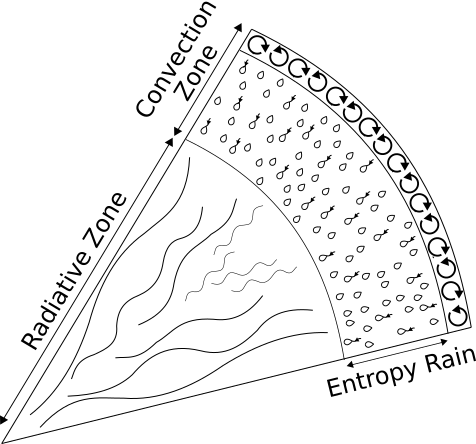
\includegraphics[width=0.32\textwidth]{./figs/entropy_rain_schematic.png}
	\vspace{-16pt}
	\end{center}
    \caption{
	A schematic of the interior of solar-type stars under the entropy rain hypothesis, where cold droplets of fluid carry the stellar luminosity below a small traditional convective surface layer.
	\label{fig:entropy_rain} }
	\vspace{-16pt}
\end{wrapfigure}

Convection which occurs in the presence of atmospheric density stratification exhibits asymmetrical upflows and downflows.
Upwellings are slow, weak, and wide while downflows are intense, fast, and narrow.
The ``entropy rain'' hypothesis \citep[][]{spruit1997} posits that downflows alone may be sufficiently powerful in stellar envelope convection to transport the stellar luminosity.
Upflows with negligible energy transport would exist alongside these downflows mostly to conserve mass.
This hypothesis, and the nontraditional dynamical form of convection it suggests, could explain the absence of giant cells in observations.
A schematic of the entropy rain picture is shown in Fig.~\ref{fig:entropy_rain}.
Recent simulations of envelope convection suggest that surface-driven downflows can transport most of the stellar luminosity \citep{kapyla&all2017}, and a modified nonlocal MLT with entropy rain was recently derived by \citet{brandenburg2016}.


\paragraph{Incorporation into MESA and Studies of Individual Raindrops} 
As a postdoctoral scholar at KITP, I will incorporate a modified MLT with nonlocal heat transport from entropy rain into MESA.
Such a modified MLT was preliminarily derived by \citet{brandenburg2016}.
I will study how nonlocal transport by downflows alters the stability of the lower convective envelope to see if entropy rain processes stabilize the deep convection zone and suppress the driving of giant cells.

While \citet{brandenburg2016}'s work will be an excellent starting point, the dynamical nature of entropy rain is not fully understood.
The downflows which constitute entropy rain may turbulently
\begin{wrapfigure}{r}{0.24\textwidth}
	\begin{center}
	\vspace{-28pt}
    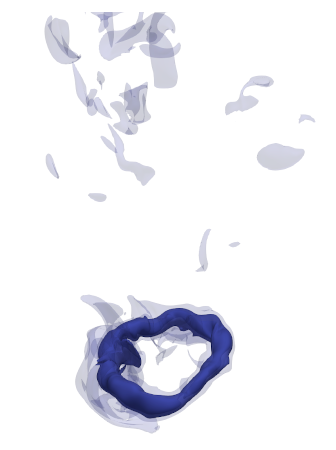
\includegraphics[width=0.22\textwidth]{./figs/turbulent_thermal.png}
	\vspace{-16pt}
	\end{center}
    \caption{
	A 3D visualization of entropy perturbations within the downward-propagating reference frame of a turbulent thermal, which may be the dynamical form of entropy rain.
	\label{fig:thermal} }
	\vspace{-16pt}
\end{wrapfigure}
break up into distinct pieces as they fall and these individual pieces can be modeled as ``thermals,'' which are observed and studied in the Earth's atmosphere \citep{lecoanet&jeevanjee2019}.
Thermals are regions of cold fluid which accelerate due to buoyancy forces and shape themselves into vortex rings; an evolved turbulent thermal is visualized in Fig.~\ref{fig:thermal}.
In \citet{andersLB2019}, I studied thermals-as-downflows in the stellar context and learned how an atmospheric density stratification affects the size of thermals as they propagate.
Over the course of my time at KITP, I will continue to study thermals to learn how to improve an MLT-with-entropy-rain.
These studies will constrain how to parameterize complex phenomena including but not limited to how effectively entropy rain overshoots into a stable radiative zone.


\section*{\textbf{Coupling MESA with Global Simulations}}
\paragraph{Context}
Modern ``321D'' \citep[e.g.,][]{arnett&all2015} studies seek to replace parameterizations like MLT with sampled statistics from fully convective, three-dimensional (3D) global simulations.
Recently, to great success, \citet{jorgensen&weiss2019} coupled 1D models to previously-computed 3D spherical shell simulations of convection in thin, near-surface layers.
Such a coupling has not yet been performed for deep convection, where most disagreements between simulations and observations occur \citep[the Convective Conundrum,][]{hanasoge&all2015}.

\paragraph{Global Scale Convection: Relaxed Dynamics}
In deep, turbulent convection, many overturn timescales pass during one Kelvin-Helmholtz (KH) timescale of atmospheric equilibration.
This long KH timescale enforces a long and scientifically-uninteresting thermal rundown on simulations of deep convection before convective statistics can be sampled.
It is therefore too computationally expensive to  
\begin{wrapfigure}{l}{0.3\textwidth}
	\begin{center}
	\vspace{-20pt}
    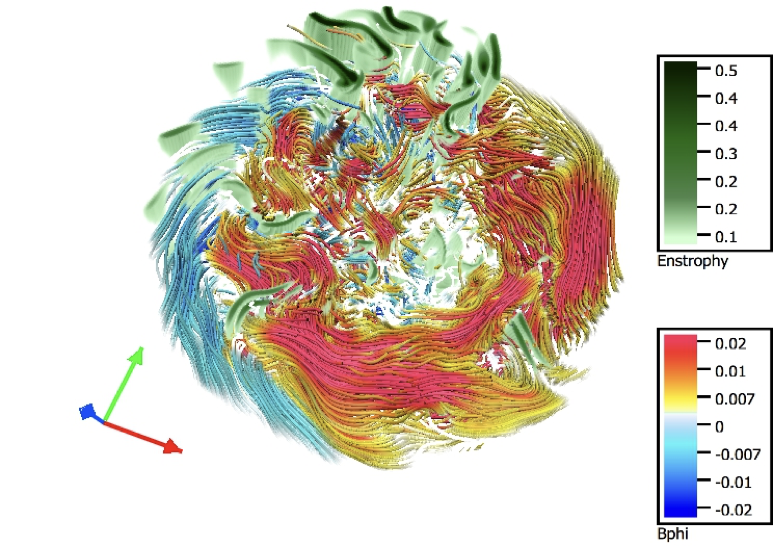
\includegraphics[width=0.28\textwidth]{./figs/mdwarf.png}
	\vspace{-16pt}
	\end{center}
    \caption{A volume rendering of a global dynamo simulation in Dedalus.
	Enstrophy, or the magnitude of vorticity, is shown in green.
	Red and blue lines denote the magnitude and direction of azimuthal magnetic field.
	\label{fig:mdwarf} }
	\vspace{-16pt}
\end{wrapfigure}
create simulations of deep convection for arbitrary stars which can be coupled with 1D models.
In \citet{anders&all2018}, I found a mechanism for fast-forwarding through the KH timescale in a simple convective system.
I verified that my fast-forwarding procedure produced the same results as standard timestepping techniques to within 1\%.
This accuracy was achieved using an order of magnitude fewer cpu-hours than traditional techniques.
As a KITP scholar, I will extend this ``Accelerated Evolution'' method \citep{anders&all2018} to global simulations by creating and validating a generalized public module which rapidly equilibrates mean thermodynamic profiles and flows.
I will use Dedalus to test the accuracy of this tool; Dedalus can simulate deep convective motions in domains that include the origin at $r = 0$ \citep[as visualized in Fig.~\ref{fig:mdwarf}, and tested in][]{lecoanet&all2019}.

\paragraph{Benchmark Main Sequence Models with 3D Convection}
As a KITP scholar, I will create an open source module which couples MESA and 3D global simulations in Dedalus.
%I will use this module to create benchmark structure profiles of main sequence stars which are informed by sampled statistics of thermally equilibrated, 3D convection.
Given a MESA stellar structure profile, this module will locate and simulate regions of convection in those profiles.
After achieving rapid thermal equilibration using the tool described in the previous section, statistics from these simulations will be fed back into MESA to update the structure.

Stellar structure is fairly time-stationary over many KH timescales during the main sequence.
As a result, a suite of main sequence stellar structure profiles which are informed by statistics from convective simulations can be feasibly constructed.
With my MESA-Dedalus module, I will generate structure profiles of stars across the main sequence, ranging from low mass, fully convective stars to high mass stars with convective cores.
These profiles will be built using statistics from 3D convection and will be made available for observers to utilize in future asteroseismic inversions.
In my own research, I will use these profiles to learn the ways in which ``true'' convection and MLT most strongly disagree in establishing a star's interior structure.

\section*{\textbf{Perspectives \& the road forward}}
With more than $10^4$ asteroseismic target stars currently available and an estimated $10^6$ available by 2030 \citep{huber&all2019}, it is critical that we solve the Convective Conundrum to properly utilize this wealth of data.
It is clear that our understanding of stellar convection is flawed, but the degree to which this flawed understanding affects asteroseismic measurements is not yet clear.
These studies proposed here will not only help to explore possible solutions to the Convective Conundrum, but will also help quantify the amount of error that imperfect convective models like MLT introduce into stellar structure codes.
The successful completion of this work will furthermore provide a set of stellar structure models which are built on sampled convective statistics, and an open source tool for arbitrarily creating these models.
I look forward to the opportunity to join Prof.~Bildsten's group to explore these questions into the Convective Conundrum and to broaden my research to explorations of other asteroseismically-motivated problems.

\bibliographystyle{yahapj}
\bibliography{biblio}
\end{document}
